\documentclass{article}
\usepackage{fixltx2e}
\usepackage{booktabs}
\usepackage{expex}
\usepackage{amssymb}
\usepackage{paralist}
\usepackage{fontspec}

\setmainfont{Linux Libertine}

\usepackage{tikz}
\usetikzlibrary{shapes,arrows,decorations.markings}
\usepackage{tikz-qtree}
\usepackage{hyperref}
\hypersetup{colorlinks,urlcolor=black,linkcolor=black,citecolor=black}

\usepackage[margin=1in]{geometry}
\usepackage{multicol}

\usepackage[hyperref=true,style=authoryear-comp,%
dashed=false,mergedate=minimum,maxbibnames=999]{biblatex}
\addbibresource{~/papers/papers.bib}
\addbibresource{biblio.bib}

\title{Persistence as a diagnostic of grammatical status: The case of
    Middle English negation (EXTENDED ABSTRACT)}
\author{Aaron Ecay and Meredith Tamminga}

\begin{document}

\maketitle

\section{Introduction}
\label{sec:introduction}

Diachronic generative syntax encompasses both the study of the syntactic
grammar of now-extinct language varieties and of the processes by which
syntactic grammars change.  In both modes of inquiry, it is necessary to
draw conclusions about the grammar of a language which no longer has any
native speakers; investigators’ only recourse is to written productions
of past native speakers.

\subsection{The Constant Rate Hypothesis}
\label{sec:const-rate-hypoth}

One tool which is available to bridge the inferential gap between the
available evidence and the desired conclusions is the Constant Rate
Hypothesis \parencite[CRH][]{Kroch1989}.  The CRH is based on the
intuition that, if there is a single grammatical cause underlying
a spectrum of surface phenomena, then these phenomena will fail to
evolve in entirely independent ways, but rather will show some common
evolutionary behavior.  Concretely, the CRH says that surface phenomena
which are governed by a single grammatical option will evolve with
parallel slopes (in the logistic-transformed domain); the single slope
reflects the advance or retreat of the governing grammatical option in
the population of authors from which observations are drawn.

% The CRH can be used to establish identity between two
% seemingly-disparate surface phenomena.  This was the use to which
% \textcite{Kroch1989} put the principle in arguing that \emph{do}-support
% and the movement of a lexical verb past the adverb \emph{never} were
% reflexes of a single grammatical parameter (governing verb movement).
% The CRH can also be used to establish that two phenomena are
% unrelated. % TODO: example here.

% The statistical tests that undergird the use of the CRH in diachronic
% inquiry are not a magic bullet; they cannot of themselves conclusively
% answer questions of grammatical (non)identity or structure.  This
% limitation stems from several factors.  One has to do with the nature of
% the statistical tests themselves: standard formulations of the tests can
% only detect when a true difference is likely to exist; they do not
% distinguish between the lack of a true difference and the lack of
% sufficient evidence to make a determination.  The second has to do with
% another aspect of the statistical procedure.  Since statistical tests of
% the CRH are embedded in a wider regression model, the outcomes of those
% tests are conditional on the (non)inclusion of other predictors in the
% model.  Stated another way, we virtually never expect to see exact
% identity of slopes to spring from raw data; confounding factors must
% first be removed.  The specifics of this de-confounnding have the
% potential to alter the results of the inquiry.  Finally, the application
% of tests of the CRH is always guided by a research agenda which includes
% information from other modes of inquiry; this other information
% contributes to the success of the CRH as a diagnostic tool by allowing
% it to apply to situations where it is likely to succeed in either
% confirming or disconfirming a salient question.

\subsection{Persistence}
\label{sec:persist}

\textcite{Sankoff:1978} observed that individual observations (tokens)
of variable linguistic phenomena are not independent of each other.  One
facet of this non-independence is \emph{persistence}: the tendency of
speakers to repeat the same linguistic option in natural speech.  The
phenomenon of persistence itself has been the object of study.  An
extensive experimental literature beginning with \textcite{Bock:1986}
demonstrates that abstract syntactic structures (and not merely words or
sounds) can be persistent.  Persistence has also been studied in
corpora, both written and spoken.  Morphosyntactic features such as
number agreement inside Spanish DPs \parencite{Poplack:1980} and the
English passive alternation \parencite{Weiner:1983} have been observed
to be subject to persistence in spoken corpora.  \textcite{Gries:2005}
compares persistence effects in both written and spoken corpora with
those observed experimentally, and finds them to be consistent with each
other.

The existence of persistence effects has been used to argue for the
existence of shared structure between surface variants.  In the words of
\textcite[490]{Branigan:1995}, “If the processing of a stimulus affects
the processing of another stimulus, then the two stimuli must be related
[...] if the relationship between the two stimuli is syntactic, then we
can use this relationship as a way of understanding what syntactic
information is represented.”  \textcite{Estival:1985} studied two
different types of Modern English passives (lexical vs.\
transformational),
% in a corpus of...writing or speech?
and found that each type facilitates itself but not the other.
% This is illustrated in figure 1...
Though the details of syntactic theories of passive formation have
changed in the intervening 30 years, modern theories \parencite[such
as][]{Embick:2004} maintain a distinction between these two types – and
indeed must do so, in view of Estival’s evidence.

% Bock on dbl obj alternation; ferreira on C vs D that – mention these here?

\subsection{The present study}
\label{sec:present-study}

In this paper, we will propose the study of persistence data from a
historical corpus to augment the study of a syntactic change.  We argue
that persistence serves as a lever which allows the force of
quantitative language use data to move forward the inquiry into
syntactic structures.  It thus joins the CRH as a useful, indeed vital,
tool for diachronic syntacticians.

% TODO: expand

\section{Middle English negation}
\label{sec:middle-engl-negat}

\begin{figure}
    \centering
    % Created by tikzDevice version 0.6.2-92-0ad2792 on 2013-07-31 01:59:21
% !TEX encoding = UTF-8 Unicode
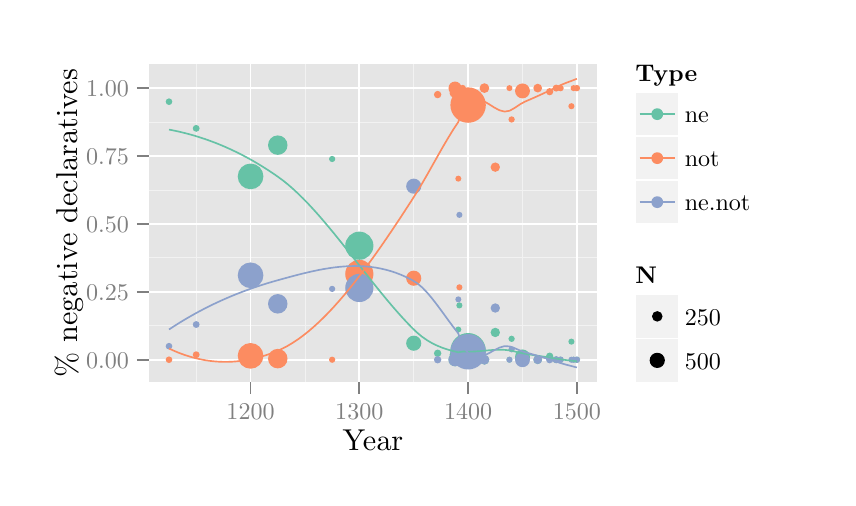
\begin{tikzpicture}[x=1pt,y=1pt]
\definecolor[named]{fillColor}{rgb}{1.00,1.00,1.00}
\path[use as bounding box,fill=fillColor,fill opacity=0.00] (0,0) rectangle (289.08,162.61);
\begin{scope}
\path[clip] (  0.00,  0.00) rectangle (289.08,162.61);
\definecolor[named]{drawColor}{rgb}{1.00,1.00,1.00}
\definecolor[named]{fillColor}{rgb}{1.00,1.00,1.00}

\path[draw=drawColor,line width= 0.6pt,line join=round,line cap=round,fill=fillColor] ( -0.00,  0.00) rectangle (289.08,162.61);
\end{scope}
\begin{scope}
\path[clip] ( 43.70, 34.60) rectangle (205.82,149.36);
\definecolor[named]{fillColor}{rgb}{0.90,0.90,0.90}

\path[fill=fillColor] ( 43.70, 34.60) rectangle (205.82,149.36);
\definecolor[named]{drawColor}{rgb}{0.95,0.95,0.95}

\path[draw=drawColor,line width= 0.3pt,line join=round] ( 43.70, 54.89) --
	(205.82, 54.89);

\path[draw=drawColor,line width= 0.3pt,line join=round] ( 43.70, 79.42) --
	(205.82, 79.42);

\path[draw=drawColor,line width= 0.3pt,line join=round] ( 43.70,103.96) --
	(205.82,103.96);

\path[draw=drawColor,line width= 0.3pt,line join=round] ( 43.70,128.50) --
	(205.82,128.50);

\path[draw=drawColor,line width= 0.3pt,line join=round] ( 60.89, 34.60) --
	( 60.89,149.36);

\path[draw=drawColor,line width= 0.3pt,line join=round] (100.19, 34.60) --
	(100.19,149.36);

\path[draw=drawColor,line width= 0.3pt,line join=round] (139.50, 34.60) --
	(139.50,149.36);

\path[draw=drawColor,line width= 0.3pt,line join=round] (178.80, 34.60) --
	(178.80,149.36);
\definecolor[named]{drawColor}{rgb}{1.00,1.00,1.00}

\path[draw=drawColor,line width= 0.6pt,line join=round] ( 43.70, 42.62) --
	(205.82, 42.62);

\path[draw=drawColor,line width= 0.6pt,line join=round] ( 43.70, 67.15) --
	(205.82, 67.15);

\path[draw=drawColor,line width= 0.6pt,line join=round] ( 43.70, 91.69) --
	(205.82, 91.69);

\path[draw=drawColor,line width= 0.6pt,line join=round] ( 43.70,116.23) --
	(205.82,116.23);

\path[draw=drawColor,line width= 0.6pt,line join=round] ( 43.70,140.77) --
	(205.82,140.77);

\path[draw=drawColor,line width= 0.6pt,line join=round] ( 80.54, 34.60) --
	( 80.54,149.36);

\path[draw=drawColor,line width= 0.6pt,line join=round] (119.84, 34.60) --
	(119.84,149.36);

\path[draw=drawColor,line width= 0.6pt,line join=round] (159.15, 34.60) --
	(159.15,149.36);

\path[draw=drawColor,line width= 0.6pt,line join=round] (198.45, 34.60) --
	(198.45,149.36);
\definecolor[named]{fillColor}{rgb}{0.40,0.76,0.65}

\path[fill=fillColor] ( 51.07,135.86) circle (  1.20);

\path[fill=fillColor] ( 60.89,126.23) circle (  1.24);

\path[fill=fillColor] ( 80.54,108.86) circle (  4.64);

\path[fill=fillColor] ( 90.37,120.16) circle (  3.52);

\path[fill=fillColor] (110.02,115.16) circle (  1.13);

\path[fill=fillColor] (119.84, 83.82) circle (  5.09);

\path[fill=fillColor] (139.50, 48.59) circle (  2.73);

\path[fill=fillColor] (148.14, 44.95) circle (  1.34);

\path[fill=fillColor] (154.04, 44.41) circle (  1.61);

\path[fill=fillColor] (154.43, 42.62) circle (  2.37);

\path[fill=fillColor] (155.61, 53.52) circle (  1.09);

\path[fill=fillColor] (156.00, 62.25) circle (  1.11);

\path[fill=fillColor] (157.18, 42.62) circle (  1.18);

\path[fill=fillColor] (157.57, 49.89) circle (  1.14);

\path[fill=fillColor] (159.15, 45.87) circle (  6.40);

\path[fill=fillColor] (165.04, 42.62) circle (  1.76);

\path[fill=fillColor] (168.97, 52.48) circle (  1.70);

\path[fill=fillColor] (174.08, 42.62) circle (  1.09);

\path[fill=fillColor] (174.87, 50.17) circle (  1.14);

\path[fill=fillColor] (178.80, 43.64) circle (  2.69);

\path[fill=fillColor] (179.58, 42.62) circle (  1.07);

\path[fill=fillColor] (184.30, 42.62) circle (  1.58);

\path[fill=fillColor] (188.62, 43.91) circle (  1.31);

\path[fill=fillColor] (190.98, 42.62) circle (  1.27);

\path[fill=fillColor] (192.55, 42.62) circle (  1.16);

\path[fill=fillColor] (196.48, 49.16) circle (  1.11);

\path[fill=fillColor] (197.27, 42.62) circle (  1.10);

\path[fill=fillColor] (198.45, 42.62) circle (  1.16);
\definecolor[named]{fillColor}{rgb}{0.99,0.55,0.38}

\path[fill=fillColor] ( 51.07, 42.62) circle (  1.20);

\path[fill=fillColor] ( 60.89, 44.43) circle (  1.24);

\path[fill=fillColor] ( 80.54, 44.02) circle (  4.64);

\path[fill=fillColor] ( 90.37, 43.02) circle (  3.52);

\path[fill=fillColor] (110.02, 42.62) circle (  1.13);

\path[fill=fillColor] (119.84, 73.62) circle (  5.09);

\path[fill=fillColor] (139.50, 72.08) circle (  2.73);

\path[fill=fillColor] (148.14,138.43) circle (  1.34);

\path[fill=fillColor] (154.04,138.97) circle (  1.61);

\path[fill=fillColor] (154.43,140.77) circle (  2.37);

\path[fill=fillColor] (155.61,108.05) circle (  1.09);

\path[fill=fillColor] (156.00, 68.79) circle (  1.11);

\path[fill=fillColor] (157.18,140.77) circle (  1.18);

\path[fill=fillColor] (157.57,133.50) circle (  1.14);

\path[fill=fillColor] (159.15,134.64) circle (  6.40);

\path[fill=fillColor] (165.04,140.77) circle (  1.76);

\path[fill=fillColor] (168.97,112.21) circle (  1.70);

\path[fill=fillColor] (174.08,140.77) circle (  1.09);

\path[fill=fillColor] (174.87,129.44) circle (  1.14);

\path[fill=fillColor] (178.80,139.75) circle (  2.69);

\path[fill=fillColor] (179.58,140.77) circle (  1.07);

\path[fill=fillColor] (184.30,140.77) circle (  1.58);

\path[fill=fillColor] (188.62,139.48) circle (  1.31);

\path[fill=fillColor] (190.98,140.77) circle (  1.27);

\path[fill=fillColor] (192.55,140.77) circle (  1.16);

\path[fill=fillColor] (196.48,134.23) circle (  1.11);

\path[fill=fillColor] (197.27,140.77) circle (  1.10);

\path[fill=fillColor] (198.45,140.77) circle (  1.16);
\definecolor[named]{fillColor}{rgb}{0.55,0.63,0.80}

\path[fill=fillColor] ( 51.07, 47.52) circle (  1.20);

\path[fill=fillColor] ( 60.89, 55.34) circle (  1.24);

\path[fill=fillColor] ( 80.54, 73.13) circle (  4.64);

\path[fill=fillColor] ( 90.37, 62.82) circle (  3.52);

\path[fill=fillColor] (110.02, 68.22) circle (  1.13);

\path[fill=fillColor] (119.84, 68.56) circle (  5.09);

\path[fill=fillColor] (139.50,105.33) circle (  2.73);

\path[fill=fillColor] (148.14, 42.62) circle (  1.34);

\path[fill=fillColor] (154.04, 42.62) circle (  1.61);

\path[fill=fillColor] (154.43, 42.62) circle (  2.37);

\path[fill=fillColor] (155.61, 64.43) circle (  1.09);

\path[fill=fillColor] (156.00, 94.96) circle (  1.11);

\path[fill=fillColor] (157.18, 42.62) circle (  1.18);

\path[fill=fillColor] (157.57, 42.62) circle (  1.14);

\path[fill=fillColor] (159.15, 45.49) circle (  6.40);

\path[fill=fillColor] (165.04, 42.62) circle (  1.76);

\path[fill=fillColor] (168.97, 61.31) circle (  1.70);

\path[fill=fillColor] (174.08, 42.62) circle (  1.09);

\path[fill=fillColor] (174.87, 46.39) circle (  1.14);

\path[fill=fillColor] (178.80, 42.62) circle (  2.69);

\path[fill=fillColor] (179.58, 42.62) circle (  1.07);

\path[fill=fillColor] (184.30, 42.62) circle (  1.58);

\path[fill=fillColor] (188.62, 42.62) circle (  1.31);

\path[fill=fillColor] (190.98, 42.62) circle (  1.27);

\path[fill=fillColor] (192.55, 42.62) circle (  1.16);

\path[fill=fillColor] (196.48, 42.62) circle (  1.11);

\path[fill=fillColor] (197.27, 42.62) circle (  1.10);

\path[fill=fillColor] (198.45, 42.62) circle (  1.16);
\definecolor[named]{drawColor}{rgb}{0.40,0.76,0.65}

\path[draw=drawColor,line width= 0.6pt,line join=round] ( 51.07,125.79) --
	( 52.93,125.42) --
	( 54.80,125.01) --
	( 56.66,124.56) --
	( 58.53,124.07) --
	( 60.40,123.54) --
	( 62.26,122.96) --
	( 64.13,122.35) --
	( 65.99,121.68) --
	( 67.86,120.98) --
	( 69.72,120.23) --
	( 71.59,119.43) --
	( 73.45,118.59) --
	( 75.32,117.70) --
	( 77.19,116.77) --
	( 79.05,115.79) --
	( 80.92,114.76) --
	( 82.78,113.68) --
	( 84.65,112.55) --
	( 86.51,111.37) --
	( 88.38,110.15) --
	( 90.24,108.87) --
	( 92.11,107.50) --
	( 93.98,106.01) --
	( 95.84,104.39) --
	( 97.71,102.66) --
	( 99.57,100.83) --
	(101.44, 98.90) --
	(103.30, 96.89) --
	(105.17, 94.80) --
	(107.03, 92.64) --
	(108.90, 90.42) --
	(110.77, 88.16) --
	(112.63, 85.85) --
	(114.50, 83.52) --
	(116.36, 81.16) --
	(118.23, 78.78) --
	(120.09, 76.40) --
	(121.96, 74.03) --
	(123.82, 71.67) --
	(125.69, 69.33) --
	(127.56, 67.02) --
	(129.42, 64.75) --
	(131.29, 62.53) --
	(133.15, 60.37) --
	(135.02, 58.27) --
	(136.88, 56.25) --
	(138.75, 54.31) --
	(140.61, 52.51) --
	(142.48, 50.96) --
	(144.35, 49.65) --
	(146.21, 48.56) --
	(148.08, 47.66) --
	(149.94, 46.91) --
	(151.81, 46.29) --
	(153.67, 45.77) --
	(155.54, 45.32) --
	(157.40, 45.60) --
	(159.27, 45.53) --
	(161.14, 45.57) --
	(163.00, 45.70) --
	(164.87, 45.87) --
	(166.73, 46.04) --
	(168.60, 46.18) --
	(170.46, 46.24) --
	(172.33, 46.19) --
	(174.19, 45.98) --
	(176.06, 45.58) --
	(177.93, 45.12) --
	(179.79, 44.76) --
	(181.66, 44.47) --
	(183.52, 44.19) --
	(185.39, 43.90) --
	(187.25, 43.61) --
	(189.12, 43.31) --
	(190.99, 43.02) --
	(192.85, 42.73) --
	(194.72, 42.48) --
	(196.58, 42.27) --
	(198.45, 42.05);
\definecolor[named]{drawColor}{rgb}{0.99,0.55,0.38}

\path[draw=drawColor,line width= 0.6pt,line join=round] ( 51.07, 46.67) --
	( 52.93, 45.82) --
	( 54.80, 45.05) --
	( 56.66, 44.37) --
	( 58.53, 43.77) --
	( 60.40, 43.25) --
	( 62.26, 42.81) --
	( 64.13, 42.45) --
	( 65.99, 42.18) --
	( 67.86, 41.99) --
	( 69.72, 41.87) --
	( 71.59, 41.84) --
	( 73.45, 41.88) --
	( 75.32, 42.01) --
	( 77.19, 42.21) --
	( 79.05, 42.49) --
	( 80.92, 42.86) --
	( 82.78, 43.29) --
	( 84.65, 43.81) --
	( 86.51, 44.40) --
	( 88.38, 45.07) --
	( 90.24, 45.82) --
	( 92.11, 46.67) --
	( 93.98, 47.65) --
	( 95.84, 48.77) --
	( 97.71, 50.01) --
	( 99.57, 51.38) --
	(101.44, 52.86) --
	(103.30, 54.46) --
	(105.17, 56.16) --
	(107.03, 57.97) --
	(108.90, 59.87) --
	(110.77, 61.88) --
	(112.63, 63.97) --
	(114.50, 66.14) --
	(116.36, 68.40) --
	(118.23, 70.74) --
	(120.09, 73.15) --
	(121.96, 75.62) --
	(123.82, 78.16) --
	(125.69, 80.76) --
	(127.56, 83.41) --
	(129.42, 86.11) --
	(131.29, 88.86) --
	(133.15, 91.64) --
	(135.02, 94.46) --
	(136.88, 97.32) --
	(138.75,100.20) --
	(140.61,103.14) --
	(142.48,106.24) --
	(144.35,109.47) --
	(146.21,112.77) --
	(148.08,116.09) --
	(149.94,119.37) --
	(151.81,122.56) --
	(153.67,125.61) --
	(155.54,128.44) --
	(157.40,133.15) --
	(159.27,135.58) --
	(161.14,136.65) --
	(163.00,136.70) --
	(164.87,136.03) --
	(166.73,134.95) --
	(168.60,133.76) --
	(170.46,132.77) --
	(172.33,132.28) --
	(174.19,132.60) --
	(176.06,133.66) --
	(177.93,134.93) --
	(179.79,135.93) --
	(181.66,136.73) --
	(183.52,137.55) --
	(185.39,138.40) --
	(187.25,139.27) --
	(189.12,140.16) --
	(190.99,141.06) --
	(192.85,141.96) --
	(194.72,142.73) --
	(196.58,143.41) --
	(198.45,144.14);
\definecolor[named]{drawColor}{rgb}{0.55,0.63,0.80}

\path[draw=drawColor,line width= 0.6pt,line join=round] ( 51.07, 53.55) --
	( 52.93, 54.76) --
	( 54.80, 55.94) --
	( 56.66, 57.07) --
	( 58.53, 58.16) --
	( 60.40, 59.22) --
	( 62.26, 60.23) --
	( 64.13, 61.20) --
	( 65.99, 62.14) --
	( 67.86, 63.04) --
	( 69.72, 63.90) --
	( 71.59, 64.73) --
	( 73.45, 65.53) --
	( 75.32, 66.29) --
	( 77.19, 67.02) --
	( 79.05, 67.72) --
	( 80.92, 68.39) --
	( 82.78, 69.03) --
	( 84.65, 69.64) --
	( 86.51, 70.23) --
	( 88.38, 70.78) --
	( 90.24, 71.31) --
	( 92.11, 71.83) --
	( 93.98, 72.34) --
	( 95.84, 72.84) --
	( 97.71, 73.33) --
	( 99.57, 73.80) --
	(101.44, 74.24) --
	(103.30, 74.66) --
	(105.17, 75.05) --
	(107.03, 75.40) --
	(108.90, 75.70) --
	(110.77, 75.97) --
	(112.63, 76.18) --
	(114.50, 76.34) --
	(116.36, 76.44) --
	(118.23, 76.48) --
	(120.09, 76.45) --
	(121.96, 76.35) --
	(123.82, 76.17) --
	(125.69, 75.92) --
	(127.56, 75.57) --
	(129.42, 75.14) --
	(131.29, 74.62) --
	(133.15, 73.99) --
	(135.02, 73.27) --
	(136.88, 72.43) --
	(138.75, 71.49) --
	(140.61, 70.36) --
	(142.48, 68.81) --
	(144.35, 66.88) --
	(146.21, 64.67) --
	(148.08, 62.25) --
	(149.94, 59.72) --
	(151.81, 57.15) --
	(153.67, 54.63) --
	(155.54, 52.24) --
	(157.40, 47.26) --
	(159.27, 44.89) --
	(161.14, 43.78) --
	(163.00, 43.61) --
	(164.87, 44.11) --
	(166.73, 45.01) --
	(168.60, 46.07) --
	(170.46, 47.00) --
	(172.33, 47.54) --
	(174.19, 47.43) --
	(176.06, 46.76) --
	(177.93, 45.95) --
	(179.79, 45.32) --
	(181.66, 44.80) --
	(183.52, 44.26) --
	(185.39, 43.70) --
	(187.25, 43.13) --
	(189.12, 42.53) --
	(190.99, 41.93) --
	(192.85, 41.32) --
	(194.72, 40.79) --
	(196.58, 40.32) --
	(198.45, 39.82);
\end{scope}
\begin{scope}
\path[clip] (  0.00,  0.00) rectangle (289.08,162.61);
\definecolor[named]{drawColor}{rgb}{0.50,0.50,0.50}

\node[text=drawColor,anchor=base east,inner sep=0pt, outer sep=0pt, scale=  0.87] at ( 36.59, 39.45) {0.00};

\node[text=drawColor,anchor=base east,inner sep=0pt, outer sep=0pt, scale=  0.87] at ( 36.59, 63.99) {0.25};

\node[text=drawColor,anchor=base east,inner sep=0pt, outer sep=0pt, scale=  0.87] at ( 36.59, 88.53) {0.50};

\node[text=drawColor,anchor=base east,inner sep=0pt, outer sep=0pt, scale=  0.87] at ( 36.59,113.07) {0.75};

\node[text=drawColor,anchor=base east,inner sep=0pt, outer sep=0pt, scale=  0.87] at ( 36.59,137.60) {1.00};
\end{scope}
\begin{scope}
\path[clip] (  0.00,  0.00) rectangle (289.08,162.61);
\definecolor[named]{drawColor}{rgb}{0.50,0.50,0.50}

\path[draw=drawColor,line width= 0.6pt,line join=round] ( 39.43, 42.62) --
	( 43.70, 42.62);

\path[draw=drawColor,line width= 0.6pt,line join=round] ( 39.43, 67.15) --
	( 43.70, 67.15);

\path[draw=drawColor,line width= 0.6pt,line join=round] ( 39.43, 91.69) --
	( 43.70, 91.69);

\path[draw=drawColor,line width= 0.6pt,line join=round] ( 39.43,116.23) --
	( 43.70,116.23);

\path[draw=drawColor,line width= 0.6pt,line join=round] ( 39.43,140.77) --
	( 43.70,140.77);
\end{scope}
\begin{scope}
\path[clip] (  0.00,  0.00) rectangle (289.08,162.61);
\definecolor[named]{drawColor}{rgb}{0.50,0.50,0.50}

\path[draw=drawColor,line width= 0.6pt,line join=round] ( 80.54, 30.33) --
	( 80.54, 34.60);

\path[draw=drawColor,line width= 0.6pt,line join=round] (119.84, 30.33) --
	(119.84, 34.60);

\path[draw=drawColor,line width= 0.6pt,line join=round] (159.15, 30.33) --
	(159.15, 34.60);

\path[draw=drawColor,line width= 0.6pt,line join=round] (198.45, 30.33) --
	(198.45, 34.60);
\end{scope}
\begin{scope}
\path[clip] (  0.00,  0.00) rectangle (289.08,162.61);
\definecolor[named]{drawColor}{rgb}{0.50,0.50,0.50}

\node[text=drawColor,anchor=base,inner sep=0pt, outer sep=0pt, scale=  0.87] at ( 80.54, 21.16) {1200};

\node[text=drawColor,anchor=base,inner sep=0pt, outer sep=0pt, scale=  0.87] at (119.84, 21.16) {1300};

\node[text=drawColor,anchor=base,inner sep=0pt, outer sep=0pt, scale=  0.87] at (159.15, 21.16) {1400};

\node[text=drawColor,anchor=base,inner sep=0pt, outer sep=0pt, scale=  0.87] at (198.45, 21.16) {1500};
\end{scope}
\begin{scope}
\path[clip] (  0.00,  0.00) rectangle (289.08,162.61);
\definecolor[named]{drawColor}{rgb}{0.00,0.00,0.00}

\node[text=drawColor,anchor=base,inner sep=0pt, outer sep=0pt, scale=  1.09] at (124.76,  9.94) {Year};
\end{scope}
\begin{scope}
\path[clip] (  0.00,  0.00) rectangle (289.08,162.61);
\definecolor[named]{drawColor}{rgb}{0.00,0.00,0.00}

\node[text=drawColor,rotate= 90.00,anchor=base,inner sep=0pt, outer sep=0pt, scale=  1.09] at ( 17.85, 91.98) {\% negative declaratives};
\end{scope}
\begin{scope}
\path[clip] (  0.00,  0.00) rectangle (289.08,162.61);
\definecolor[named]{fillColor}{rgb}{1.00,1.00,1.00}

\path[fill=fillColor] (215.29, 87.34) rectangle (266.36,153.79);
\end{scope}
\begin{scope}
\path[clip] (  0.00,  0.00) rectangle (289.08,162.61);
\definecolor[named]{drawColor}{rgb}{0.00,0.00,0.00}

\node[text=drawColor,anchor=base west,inner sep=0pt, outer sep=0pt, scale=  0.87] at (219.55,143.28) {\bfseries Type};
\end{scope}
\begin{scope}
\path[clip] (  0.00,  0.00) rectangle (289.08,162.61);
\definecolor[named]{drawColor}{rgb}{1.00,1.00,1.00}
\definecolor[named]{fillColor}{rgb}{0.95,0.95,0.95}

\path[draw=drawColor,line width= 0.6pt,line join=round,line cap=round,fill=fillColor] (219.55,123.41) rectangle (235.45,139.31);
\end{scope}
\begin{scope}
\path[clip] (  0.00,  0.00) rectangle (289.08,162.61);
\definecolor[named]{fillColor}{rgb}{0.40,0.76,0.65}

\path[fill=fillColor] (227.50,131.36) circle (  2.13);
\end{scope}
\begin{scope}
\path[clip] (  0.00,  0.00) rectangle (289.08,162.61);
\definecolor[named]{drawColor}{rgb}{0.40,0.76,0.65}

\path[draw=drawColor,line width= 0.6pt,line join=round] (221.14,131.36) -- (233.86,131.36);
\end{scope}
\begin{scope}
\path[clip] (  0.00,  0.00) rectangle (289.08,162.61);
\definecolor[named]{drawColor}{rgb}{1.00,1.00,1.00}
\definecolor[named]{fillColor}{rgb}{0.95,0.95,0.95}

\path[draw=drawColor,line width= 0.6pt,line join=round,line cap=round,fill=fillColor] (219.55,107.51) rectangle (235.45,123.41);
\end{scope}
\begin{scope}
\path[clip] (  0.00,  0.00) rectangle (289.08,162.61);
\definecolor[named]{fillColor}{rgb}{0.99,0.55,0.38}

\path[fill=fillColor] (227.50,115.46) circle (  2.13);
\end{scope}
\begin{scope}
\path[clip] (  0.00,  0.00) rectangle (289.08,162.61);
\definecolor[named]{drawColor}{rgb}{0.99,0.55,0.38}

\path[draw=drawColor,line width= 0.6pt,line join=round] (221.14,115.46) -- (233.86,115.46);
\end{scope}
\begin{scope}
\path[clip] (  0.00,  0.00) rectangle (289.08,162.61);
\definecolor[named]{drawColor}{rgb}{1.00,1.00,1.00}
\definecolor[named]{fillColor}{rgb}{0.95,0.95,0.95}

\path[draw=drawColor,line width= 0.6pt,line join=round,line cap=round,fill=fillColor] (219.55, 91.61) rectangle (235.45,107.51);
\end{scope}
\begin{scope}
\path[clip] (  0.00,  0.00) rectangle (289.08,162.61);
\definecolor[named]{fillColor}{rgb}{0.55,0.63,0.80}

\path[fill=fillColor] (227.50, 99.56) circle (  2.13);
\end{scope}
\begin{scope}
\path[clip] (  0.00,  0.00) rectangle (289.08,162.61);
\definecolor[named]{drawColor}{rgb}{0.55,0.63,0.80}

\path[draw=drawColor,line width= 0.6pt,line join=round] (221.14, 99.56) -- (233.86, 99.56);
\end{scope}
\begin{scope}
\path[clip] (  0.00,  0.00) rectangle (289.08,162.61);
\definecolor[named]{drawColor}{rgb}{0.00,0.00,0.00}

\node[text=drawColor,anchor=base west,inner sep=0pt, outer sep=0pt, scale=  0.87] at (237.44,128.19) {ne};
\end{scope}
\begin{scope}
\path[clip] (  0.00,  0.00) rectangle (289.08,162.61);
\definecolor[named]{drawColor}{rgb}{0.00,0.00,0.00}

\node[text=drawColor,anchor=base west,inner sep=0pt, outer sep=0pt, scale=  0.87] at (237.44,112.29) {not};
\end{scope}
\begin{scope}
\path[clip] (  0.00,  0.00) rectangle (289.08,162.61);
\definecolor[named]{drawColor}{rgb}{0.00,0.00,0.00}

\node[text=drawColor,anchor=base west,inner sep=0pt, outer sep=0pt, scale=  0.87] at (237.44, 96.40) {ne.not};
\end{scope}
\begin{scope}
\path[clip] (  0.00,  0.00) rectangle (289.08,162.61);
\definecolor[named]{fillColor}{rgb}{1.00,1.00,1.00}

\path[fill=fillColor] (215.29, 30.17) rectangle (255.04, 80.72);
\end{scope}
\begin{scope}
\path[clip] (  0.00,  0.00) rectangle (289.08,162.61);
\definecolor[named]{drawColor}{rgb}{0.00,0.00,0.00}

\node[text=drawColor,anchor=base west,inner sep=0pt, outer sep=0pt, scale=  0.87] at (219.55, 70.21) {\bfseries N};
\end{scope}
\begin{scope}
\path[clip] (  0.00,  0.00) rectangle (289.08,162.61);
\definecolor[named]{drawColor}{rgb}{1.00,1.00,1.00}
\definecolor[named]{fillColor}{rgb}{0.95,0.95,0.95}

\path[draw=drawColor,line width= 0.6pt,line join=round,line cap=round,fill=fillColor] (219.55, 50.34) rectangle (235.45, 66.24);
\end{scope}
\begin{scope}
\path[clip] (  0.00,  0.00) rectangle (289.08,162.61);
\definecolor[named]{fillColor}{rgb}{0.00,0.00,0.00}

\path[fill=fillColor] (227.50, 58.29) circle (  1.91);
\end{scope}
\begin{scope}
\path[clip] (  0.00,  0.00) rectangle (289.08,162.61);
\definecolor[named]{drawColor}{rgb}{1.00,1.00,1.00}
\definecolor[named]{fillColor}{rgb}{0.95,0.95,0.95}

\path[draw=drawColor,line width= 0.6pt,line join=round,line cap=round,fill=fillColor] (219.55, 34.44) rectangle (235.45, 50.34);
\end{scope}
\begin{scope}
\path[clip] (  0.00,  0.00) rectangle (289.08,162.61);
\definecolor[named]{fillColor}{rgb}{0.00,0.00,0.00}

\path[fill=fillColor] (227.50, 42.39) circle (  2.75);
\end{scope}
\begin{scope}
\path[clip] (  0.00,  0.00) rectangle (289.08,162.61);
\definecolor[named]{drawColor}{rgb}{0.00,0.00,0.00}

\node[text=drawColor,anchor=base west,inner sep=0pt, outer sep=0pt, scale=  0.87] at (237.44, 55.12) {250};
\end{scope}
\begin{scope}
\path[clip] (  0.00,  0.00) rectangle (289.08,162.61);
\definecolor[named]{drawColor}{rgb}{0.00,0.00,0.00}

\node[text=drawColor,anchor=base west,inner sep=0pt, outer sep=0pt, scale=  0.87] at (237.44, 39.22) {500};
\end{scope}
\end{tikzpicture}

    % TODO: scale_size_area
    \caption{The rates of occurrence of the three types of negative sentence in Middle English, during the change from \emph{ne} to \emph{not}.  Data from the PPCME2.}
    \label{fig:three-lines}
\end{figure}

In Middle English, there is a change in the exponence of Neg, the head
which introduces sentence negation.  The negator \emph{ne}, inherited
from Old English, is lost.  The word \emph{not}, an Old English negative
adverb, becomes the new exponent of sentence negation.  While the change
is in progress, there are many tokens of sentences which have both
\emph{ne} and \emph{not}:
\ex
he ne shal nouʒt decieue him \trailingcitation{Early Prose Psalter,
    161:131:11, from \textcite{Frisch1997}}
\xe
In Figure~\ref{fig:three-lines} the change is illustrated with data from
the Penn Parsed Corpus of Middle English, version
2. \parencite[PPCME2][]{Kroch2001} The lavender line traces the rise and
disappearance of \emph{ne...not} sentences.
% TODO: won’t be lavender in the print version

\subsection{The analysis of \textcite{Frisch1997}}
\label{sec:frisch-analysis}

\begin{figure}
    \centering
    \begin{multicols}{3}
        \Tree [.TP T [.NegP [.Neg \emph{ne}\textsubscript{[+Neg]} ]
        [.VP \edge[roof]; {...} ] ] ]

        \Tree [.TP T [.NegP [.XP \emph{not}\textsubscript{[+Neg]} ]
        [.Neg$'$ [.Neg \emph{ne}\textsubscript{[+Neg]}
        ] [.VP \edge[roof]; {...} ] ] ] ]

        \Tree [.TP T [.NegP [.XP \emph{not}\textsubscript{[+Neg]} ]
        [.Neg$'$ [.Neg $\varnothing$ ]
        [.VP \edge[roof]; {...} ] ] ] ]
    \end{multicols}
    \caption{The derivation of the three types of ME negative sentence
        according to \textcite{Frisch1997}.}
    \label{fig:frisch-trees}
\end{figure}

\textcite{Frisch1997} analyzes this change to be due to
competition \parencite[in the sense of][]{Kroch1989} between two
grammars.  One grammar dictates that \emph{ne} is the exponent of
Neg$^0$; the other says that \emph{not} is merged in the specifier of
NegP, and is the (lone) exponent of that projection.  When both grammars
(really, lexical entries) are activated, the result is spelling out
Neg$^0$ as \emph{ne} and Spec,NegP as \emph{not}, leading to a surface
\emph{ne...not} sentence.  Figure~\ref{fig:frisch-trees} illustrates the
three derivations.  In this figure, the notation [+Neg] indicates a
projection which carries the semantic value of sentence negation.
Frisch invokes an auxiliary hypothesis about the structure of UG to
avoid the two negations canceling each other out in \emph{ne...not}
sentences.

% TODO: discuss evidence

\subsection{The analysis of \textcite{wallage08}}
\label{sec:wallage-analysis}

\begin{figure}
    \centering
    \begin{multicols}{3}

        \Tree [.TP T [.NegP [.Neg \emph{ne}\textsubscript{[+Neg]} ]
        [.VP \edge[roof]; {...} ] ] ]

        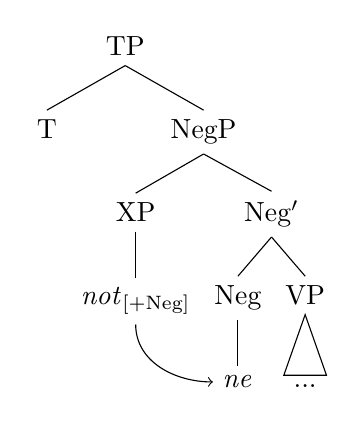
\begin{tikzpicture}{every tree node/.style={align=center,anchor=north}}
            \Tree [.TP T [.NegP [.XP
            \node(not){\emph{not}{\textsubscript{[+Neg]}}};
            ] [.Neg$'$ [.Neg \node(ne){\emph{ne}};
            ] [.VP \edge[roof]; {...} ] ] ] ]

            \draw[->] (not) to[out=-90, in=180] (ne);
        \end{tikzpicture}

        \Tree [.TP T [.NegP [.XP
        {\emph{not}{\textsubscript{[+Neg]}}} ]
        [.Neg$'$ [.Neg $\varnothing$ ] [.VP \edge[roof]; {...} ] ] ] ]
    \end{multicols}
    \caption{The derivation of the three types of ME negative sentence
        according to \textcite{wallage08}.}
    \label{fig:wallage-trees}
\end{figure}

\textcite{wallage08} analyzes the change in a different way, taking as a
point of departure Jespersen’s Cycle, %TODO: cite
a cross-linguistically well-attested generalization about the evolution
of negation.  Wallage posits that the Cycle is operative in ME, and that
\emph{ne}, \emph{ne...not} and \emph{not} are each stages in the cycle,
each with a separate grammatical existence from the others.  In
\emph{ne...not} type constructions, according to Wallage, \emph{ne} is
bereft of negative force, and is rather generated by negative concord.
This analysis is shown in Figure~\ref{fig:wallage-trees}.

% TODO: Wallage’s evidence

\subsection{Summary}
\label{sec:summary}

There is a fundamental disagreement between Frisch and Wallage about the
grammatical structures at play during the ME negation change.  This
disagreement boils down to the question of whether there were two
grammatical structures interacting (to wit \emph{ne} and \emph{not}), or
three (the former two plus \emph{ne...not}).  There is evidence to
support each position based on the CRH.  Wallage has questioned
the value of Frisch’s evidence on grounds having to do with (inter alia)
main vs.\ embedded clause distinctions.  It is possible that this
criticism is well-taken.  But there is a subtle danger.  The more that
the data are re-examined and the larger the auxiliary structure of
corrections and transformations of the raw data grows, the more fragile
the CRH result becomes.  (This is an especially acute problem in the
case of Middle English, where most of the available data have already
been incorporated into the analysis.  Work on later stages of English
allows the possibility of testing hypotheses on newly-collected
corpora).

We propose to examine the existing data from the point of view of
persistence.  Just like the CRH, persistence phenomena allow us to use
statistical patterns to argue for or against hypotheses about
grammatical representations.    % ... TODO: move to conclusion

\section{Results}
\label{sec:results}

In order to undertake our investgation, we assembled a corpus of
consecutive negative declarative clauses in the PPCME2.  We allowed the
clauses to be at any distance from each other, but required that there
not be any intervening “spurious” negation.\footnote{For our purposes,
    spurious negation consists of:
    \begin{inparaitem}
      \item contracted \emph{ne}, as in \emph{nis}, \emph{naere}, etc.
      \item negative quantifiers (\emph{none}) and adverbs
        (\emph{never}), whether or not they trigger negative concord
      \item \emph{not only...} constructions, and
      \item (possible) constituent negation of a verb or adverb, as in
        \emph{John might eat but not drink} or \emph{John might not
            frequently eat}.
    \end{inparaitem}
}
Most negative sentences not thus excluded will be counted twice: once as
a prime (first member of a pair) and once as a target (second member).
(The first/last sentence of a text and sentences just after/before a
token of spurious negation will be counted only once, as a prime/target
respectively.)  The corpus contains 598 target–prime pairs in the years
1250–1349 (inclusive).  This date range constitutes the middle century
of the change, when each of the three alternative surface patterns is
approximately equal in incidence.  It thus will be the most fertile
ground for the discernment of patterns, and will from the basis of the
bulk of our analysis.

\subsection{Two-atom model}
\label{sec:two-atom-model}

\begin{figure}
    \centering
    % Created by tikzDevice version 0.6.2-92-0ad2792 on 2013-07-31 02:20:55
% !TEX encoding = UTF-8 Unicode
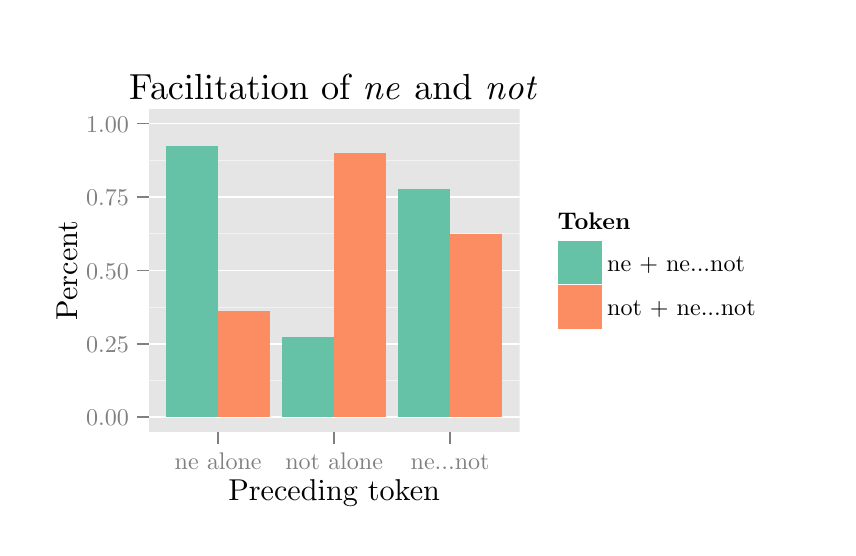
\begin{tikzpicture}[x=1pt,y=1pt]
\definecolor[named]{fillColor}{rgb}{1.00,1.00,1.00}
\path[use as bounding box,fill=fillColor,fill opacity=0.00] (0,0) rectangle (289.08,180.67);
\begin{scope}
\path[clip] (  0.00,  0.00) rectangle (289.08,180.67);
\definecolor[named]{drawColor}{rgb}{1.00,1.00,1.00}
\definecolor[named]{fillColor}{rgb}{1.00,1.00,1.00}

\path[draw=drawColor,line width= 0.6pt,line join=round,line cap=round,fill=fillColor] ( -0.00,  0.00) rectangle (289.08,180.68);
\end{scope}
\begin{scope}
\path[clip] ( 43.70, 34.60) rectangle (177.78,151.31);
\definecolor[named]{fillColor}{rgb}{0.90,0.90,0.90}

\path[fill=fillColor] ( 43.70, 34.60) rectangle (177.78,151.31);
\definecolor[named]{drawColor}{rgb}{0.95,0.95,0.95}

\path[draw=drawColor,line width= 0.3pt,line join=round] ( 43.70, 53.17) --
	(177.78, 53.17);

\path[draw=drawColor,line width= 0.3pt,line join=round] ( 43.70, 79.69) --
	(177.78, 79.69);

\path[draw=drawColor,line width= 0.3pt,line join=round] ( 43.70,106.22) --
	(177.78,106.22);

\path[draw=drawColor,line width= 0.3pt,line join=round] ( 43.70,132.74) --
	(177.78,132.74);
\definecolor[named]{drawColor}{rgb}{1.00,1.00,1.00}

\path[draw=drawColor,line width= 0.6pt,line join=round] ( 43.70, 39.90) --
	(177.78, 39.90);

\path[draw=drawColor,line width= 0.6pt,line join=round] ( 43.70, 66.43) --
	(177.78, 66.43);

\path[draw=drawColor,line width= 0.6pt,line join=round] ( 43.70, 92.95) --
	(177.78, 92.95);

\path[draw=drawColor,line width= 0.6pt,line join=round] ( 43.70,119.48) --
	(177.78,119.48);

\path[draw=drawColor,line width= 0.6pt,line join=round] ( 43.70,146.00) --
	(177.78,146.00);
\definecolor[named]{fillColor}{rgb}{0.40,0.76,0.65}

\path[fill=fillColor] ( 49.98, 39.90) rectangle ( 68.84,137.93);
\definecolor[named]{fillColor}{rgb}{0.99,0.55,0.38}

\path[fill=fillColor] ( 68.84, 39.90) rectangle ( 87.69, 78.14);
\definecolor[named]{fillColor}{rgb}{0.40,0.76,0.65}

\path[fill=fillColor] ( 91.88, 39.90) rectangle (110.74, 68.75);
\definecolor[named]{fillColor}{rgb}{0.99,0.55,0.38}

\path[fill=fillColor] (110.74, 39.90) rectangle (129.59,135.25);
\definecolor[named]{fillColor}{rgb}{0.40,0.76,0.65}

\path[fill=fillColor] (133.78, 39.90) rectangle (152.64,122.36);
\definecolor[named]{fillColor}{rgb}{0.99,0.55,0.38}

\path[fill=fillColor] (152.64, 39.90) rectangle (171.49,106.22);
\end{scope}
\begin{scope}
\path[clip] (  0.00,  0.00) rectangle (289.08,180.67);
\definecolor[named]{drawColor}{rgb}{0.50,0.50,0.50}

\node[text=drawColor,anchor=base east,inner sep=0pt, outer sep=0pt, scale=  0.87] at ( 36.59, 36.74) {0.00};

\node[text=drawColor,anchor=base east,inner sep=0pt, outer sep=0pt, scale=  0.87] at ( 36.59, 63.27) {0.25};

\node[text=drawColor,anchor=base east,inner sep=0pt, outer sep=0pt, scale=  0.87] at ( 36.59, 89.79) {0.50};

\node[text=drawColor,anchor=base east,inner sep=0pt, outer sep=0pt, scale=  0.87] at ( 36.59,116.32) {0.75};

\node[text=drawColor,anchor=base east,inner sep=0pt, outer sep=0pt, scale=  0.87] at ( 36.59,142.84) {1.00};
\end{scope}
\begin{scope}
\path[clip] (  0.00,  0.00) rectangle (289.08,180.67);
\definecolor[named]{drawColor}{rgb}{0.50,0.50,0.50}

\path[draw=drawColor,line width= 0.6pt,line join=round] ( 39.43, 39.90) --
	( 43.70, 39.90);

\path[draw=drawColor,line width= 0.6pt,line join=round] ( 39.43, 66.43) --
	( 43.70, 66.43);

\path[draw=drawColor,line width= 0.6pt,line join=round] ( 39.43, 92.95) --
	( 43.70, 92.95);

\path[draw=drawColor,line width= 0.6pt,line join=round] ( 39.43,119.48) --
	( 43.70,119.48);

\path[draw=drawColor,line width= 0.6pt,line join=round] ( 39.43,146.00) --
	( 43.70,146.00);
\end{scope}
\begin{scope}
\path[clip] (  0.00,  0.00) rectangle (289.08,180.67);
\definecolor[named]{drawColor}{rgb}{0.50,0.50,0.50}

\path[draw=drawColor,line width= 0.6pt,line join=round] ( 68.84, 30.33) --
	( 68.84, 34.60);

\path[draw=drawColor,line width= 0.6pt,line join=round] (110.74, 30.33) --
	(110.74, 34.60);

\path[draw=drawColor,line width= 0.6pt,line join=round] (152.64, 30.33) --
	(152.64, 34.60);
\end{scope}
\begin{scope}
\path[clip] (  0.00,  0.00) rectangle (289.08,180.67);
\definecolor[named]{drawColor}{rgb}{0.50,0.50,0.50}

\node[text=drawColor,anchor=base,inner sep=0pt, outer sep=0pt, scale=  0.87] at ( 68.84, 21.16) {ne alone};

\node[text=drawColor,anchor=base,inner sep=0pt, outer sep=0pt, scale=  0.87] at (110.74, 21.16) {not alone};

\node[text=drawColor,anchor=base,inner sep=0pt, outer sep=0pt, scale=  0.87] at (152.64, 21.16) {ne...not};
\end{scope}
\begin{scope}
\path[clip] (  0.00,  0.00) rectangle (289.08,180.67);
\definecolor[named]{drawColor}{rgb}{0.00,0.00,0.00}

\node[text=drawColor,anchor=base,inner sep=0pt, outer sep=0pt, scale=  1.09] at (110.74,  9.94) {Preceding token};
\end{scope}
\begin{scope}
\path[clip] (  0.00,  0.00) rectangle (289.08,180.67);
\definecolor[named]{drawColor}{rgb}{0.00,0.00,0.00}

\node[text=drawColor,rotate= 90.00,anchor=base,inner sep=0pt, outer sep=0pt, scale=  1.09] at ( 17.85, 92.95) {Percent};
\end{scope}
\begin{scope}
\path[clip] (  0.00,  0.00) rectangle (289.08,180.67);
\definecolor[named]{fillColor}{rgb}{1.00,1.00,1.00}

\path[fill=fillColor] (187.25, 67.68) rectangle (266.36,118.23);
\end{scope}
\begin{scope}
\path[clip] (  0.00,  0.00) rectangle (289.08,180.67);
\definecolor[named]{drawColor}{rgb}{0.00,0.00,0.00}

\node[text=drawColor,anchor=base west,inner sep=0pt, outer sep=0pt, scale=  0.87] at (191.52,107.72) {\bfseries Token};
\end{scope}
\begin{scope}
\path[clip] (  0.00,  0.00) rectangle (289.08,180.67);
\definecolor[named]{drawColor}{rgb}{1.00,1.00,1.00}
\definecolor[named]{fillColor}{rgb}{0.95,0.95,0.95}

\path[draw=drawColor,line width= 0.6pt,line join=round,line cap=round,fill=fillColor] (191.52, 87.85) rectangle (207.41,103.75);
\end{scope}
\begin{scope}
\path[clip] (  0.00,  0.00) rectangle (289.08,180.67);
\definecolor[named]{fillColor}{rgb}{0.40,0.76,0.65}

\path[fill=fillColor] (191.52, 87.85) rectangle (207.41,103.75);

\path[] (191.52, 87.85) --
	(207.41,103.75);
\end{scope}
\begin{scope}
\path[clip] (  0.00,  0.00) rectangle (289.08,180.67);
\definecolor[named]{drawColor}{rgb}{1.00,1.00,1.00}
\definecolor[named]{fillColor}{rgb}{0.95,0.95,0.95}

\path[draw=drawColor,line width= 0.6pt,line join=round,line cap=round,fill=fillColor] (191.52, 71.95) rectangle (207.41, 87.85);
\end{scope}
\begin{scope}
\path[clip] (  0.00,  0.00) rectangle (289.08,180.67);
\definecolor[named]{fillColor}{rgb}{0.99,0.55,0.38}

\path[fill=fillColor] (191.52, 71.95) rectangle (207.41, 87.85);

\path[] (191.52, 71.95) --
	(207.41, 87.85);
\end{scope}
\begin{scope}
\path[clip] (  0.00,  0.00) rectangle (289.08,180.67);
\definecolor[named]{drawColor}{rgb}{0.00,0.00,0.00}

\node[text=drawColor,anchor=base west,inner sep=0pt, outer sep=0pt, scale=  0.87] at (209.40, 92.63) {ne + ne...not};
\end{scope}
\begin{scope}
\path[clip] (  0.00,  0.00) rectangle (289.08,180.67);
\definecolor[named]{drawColor}{rgb}{0.00,0.00,0.00}

\node[text=drawColor,anchor=base west,inner sep=0pt, outer sep=0pt, scale=  0.87] at (209.40, 76.73) {not + ne...not};
\end{scope}
\begin{scope}
\path[clip] (  0.00,  0.00) rectangle (289.08,180.67);
\definecolor[named]{drawColor}{rgb}{0.00,0.00,0.00}

\node[text=drawColor,anchor=base,inner sep=0pt, outer sep=0pt, scale=  1.31] at (110.74,154.62) {Facilitation of \emph{ne} and \emph{not}};
\end{scope}
\end{tikzpicture}

    \caption{Predictions of the two-atom model.}
    \label{fig:two-atom}
\end{figure}

The two-atom model (the model espoused by Frisch) predicts that primes
containing \emph{ne} alone will have some facilitatory effect on the use
of \emph{ne} (whether alone or in combination with \emph{not}) in their
targets; \emph{not} alone will behave similarly.  Since a token fo
\emph{ne...not} contains on this model a complete instance of \emph{ne}
and a complete instance of \emph{not}, it should have the same effect as
\emph{ne} alone does on following \emph{ne}, and the same effect as
\emph{not} alone on following \emph{not}.

Figure~\ref{fig:two-atom} illustrates that this prediction is not borne
out.  The two pairs of bars on the left illustrate the size of the
persistence effect for \emph{ne} and \emph{not} alone, respectively.
Taking the leftmost bar group as an example, after a sentence negated
with \emph{ne} alone, the next negative has roughly a 90\% chance of
containing \emph{ne}, and only roughly a 35\% chance of containing
\emph{not}.\footnote{Following the model’s assignment of dual status,
    \emph{ne...not} sentences are counted twice; for this reason the
    percentages do not sum to 100\%.}  Under the model’s prediction, we
expect the effect of \emph{ne...not} on following negators to be just as
strong as the individual effects.  In other words, the right-hand green
bar should be just as tall as the left-most one, and the right-hand
orange bar should be as tall as the middle one, contrary to
fact. % TODO: color names...

\subsection{Three-atom model}
\label{sec:three-atom-model}

\begin{figure}
    \centering
    % Created by tikzDevice version 0.6.2-92-0ad2792 on 2013-07-31 02:20:56
% !TEX encoding = UTF-8 Unicode
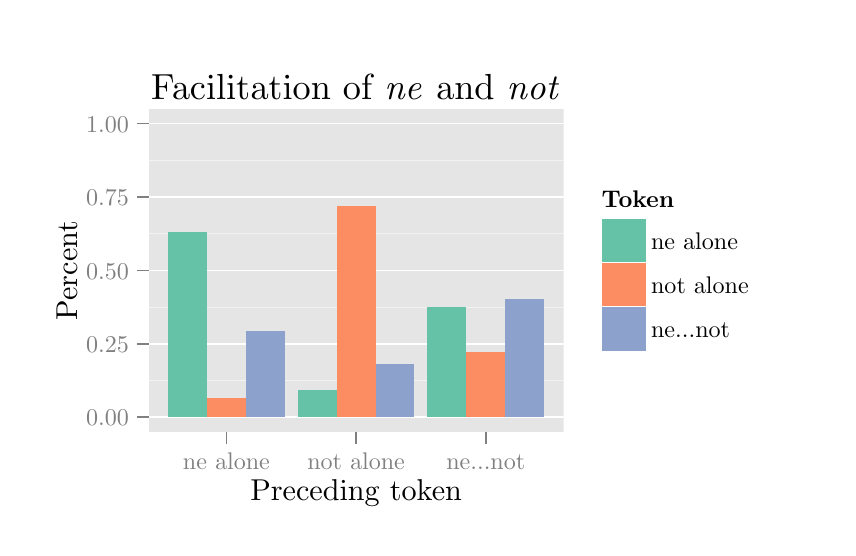
\begin{tikzpicture}[x=1pt,y=1pt]
\definecolor[named]{fillColor}{rgb}{1.00,1.00,1.00}
\path[use as bounding box,fill=fillColor,fill opacity=0.00] (0,0) rectangle (289.08,180.67);
\begin{scope}
\path[clip] (  0.00,  0.00) rectangle (289.08,180.67);
\definecolor[named]{drawColor}{rgb}{1.00,1.00,1.00}
\definecolor[named]{fillColor}{rgb}{1.00,1.00,1.00}

\path[draw=drawColor,line width= 0.6pt,line join=round,line cap=round,fill=fillColor] ( -0.00,  0.00) rectangle (289.08,180.68);
\end{scope}
\begin{scope}
\path[clip] ( 43.70, 34.60) rectangle (193.65,151.31);
\definecolor[named]{fillColor}{rgb}{0.90,0.90,0.90}

\path[fill=fillColor] ( 43.70, 34.60) rectangle (193.65,151.31);
\definecolor[named]{drawColor}{rgb}{0.95,0.95,0.95}

\path[draw=drawColor,line width= 0.3pt,line join=round] ( 43.70, 53.17) --
	(193.65, 53.17);

\path[draw=drawColor,line width= 0.3pt,line join=round] ( 43.70, 79.69) --
	(193.65, 79.69);

\path[draw=drawColor,line width= 0.3pt,line join=round] ( 43.70,106.22) --
	(193.65,106.22);

\path[draw=drawColor,line width= 0.3pt,line join=round] ( 43.70,132.74) --
	(193.65,132.74);
\definecolor[named]{drawColor}{rgb}{1.00,1.00,1.00}

\path[draw=drawColor,line width= 0.6pt,line join=round] ( 43.70, 39.90) --
	(193.65, 39.90);

\path[draw=drawColor,line width= 0.6pt,line join=round] ( 43.70, 66.43) --
	(193.65, 66.43);

\path[draw=drawColor,line width= 0.6pt,line join=round] ( 43.70, 92.95) --
	(193.65, 92.95);

\path[draw=drawColor,line width= 0.6pt,line join=round] ( 43.70,119.48) --
	(193.65,119.48);

\path[draw=drawColor,line width= 0.6pt,line join=round] ( 43.70,146.00) --
	(193.65,146.00);
\definecolor[named]{fillColor}{rgb}{0.40,0.76,0.65}

\path[fill=fillColor] ( 50.73, 39.90) rectangle ( 64.79,106.69);
\definecolor[named]{fillColor}{rgb}{0.99,0.55,0.38}

\path[fill=fillColor] ( 64.79, 39.90) rectangle ( 78.84, 46.91);
\definecolor[named]{fillColor}{rgb}{0.55,0.63,0.80}

\path[fill=fillColor] ( 78.84, 39.90) rectangle ( 92.90, 71.14);
\definecolor[named]{fillColor}{rgb}{0.40,0.76,0.65}

\path[fill=fillColor] ( 97.59, 39.90) rectangle (111.65, 49.68);
\definecolor[named]{fillColor}{rgb}{0.99,0.55,0.38}

\path[fill=fillColor] (111.65, 39.90) rectangle (125.70,116.18);
\definecolor[named]{fillColor}{rgb}{0.55,0.63,0.80}

\path[fill=fillColor] (125.70, 39.90) rectangle (139.76, 58.97);
\definecolor[named]{fillColor}{rgb}{0.40,0.76,0.65}

\path[fill=fillColor] (144.45, 39.90) rectangle (158.51, 79.69);
\definecolor[named]{fillColor}{rgb}{0.99,0.55,0.38}

\path[fill=fillColor] (158.51, 39.90) rectangle (172.56, 63.55);
\definecolor[named]{fillColor}{rgb}{0.55,0.63,0.80}

\path[fill=fillColor] (172.56, 39.90) rectangle (186.62, 82.58);
\end{scope}
\begin{scope}
\path[clip] (  0.00,  0.00) rectangle (289.08,180.67);
\definecolor[named]{drawColor}{rgb}{0.50,0.50,0.50}

\node[text=drawColor,anchor=base east,inner sep=0pt, outer sep=0pt, scale=  0.87] at ( 36.59, 36.74) {0.00};

\node[text=drawColor,anchor=base east,inner sep=0pt, outer sep=0pt, scale=  0.87] at ( 36.59, 63.27) {0.25};

\node[text=drawColor,anchor=base east,inner sep=0pt, outer sep=0pt, scale=  0.87] at ( 36.59, 89.79) {0.50};

\node[text=drawColor,anchor=base east,inner sep=0pt, outer sep=0pt, scale=  0.87] at ( 36.59,116.32) {0.75};

\node[text=drawColor,anchor=base east,inner sep=0pt, outer sep=0pt, scale=  0.87] at ( 36.59,142.84) {1.00};
\end{scope}
\begin{scope}
\path[clip] (  0.00,  0.00) rectangle (289.08,180.67);
\definecolor[named]{drawColor}{rgb}{0.50,0.50,0.50}

\path[draw=drawColor,line width= 0.6pt,line join=round] ( 39.43, 39.90) --
	( 43.70, 39.90);

\path[draw=drawColor,line width= 0.6pt,line join=round] ( 39.43, 66.43) --
	( 43.70, 66.43);

\path[draw=drawColor,line width= 0.6pt,line join=round] ( 39.43, 92.95) --
	( 43.70, 92.95);

\path[draw=drawColor,line width= 0.6pt,line join=round] ( 39.43,119.48) --
	( 43.70,119.48);

\path[draw=drawColor,line width= 0.6pt,line join=round] ( 39.43,146.00) --
	( 43.70,146.00);
\end{scope}
\begin{scope}
\path[clip] (  0.00,  0.00) rectangle (289.08,180.67);
\definecolor[named]{drawColor}{rgb}{0.50,0.50,0.50}

\path[draw=drawColor,line width= 0.6pt,line join=round] ( 71.81, 30.33) --
	( 71.81, 34.60);

\path[draw=drawColor,line width= 0.6pt,line join=round] (118.67, 30.33) --
	(118.67, 34.60);

\path[draw=drawColor,line width= 0.6pt,line join=round] (165.54, 30.33) --
	(165.54, 34.60);
\end{scope}
\begin{scope}
\path[clip] (  0.00,  0.00) rectangle (289.08,180.67);
\definecolor[named]{drawColor}{rgb}{0.50,0.50,0.50}

\node[text=drawColor,anchor=base,inner sep=0pt, outer sep=0pt, scale=  0.87] at ( 71.81, 21.16) {ne alone};

\node[text=drawColor,anchor=base,inner sep=0pt, outer sep=0pt, scale=  0.87] at (118.67, 21.16) {not alone};

\node[text=drawColor,anchor=base,inner sep=0pt, outer sep=0pt, scale=  0.87] at (165.54, 21.16) {ne...not};
\end{scope}
\begin{scope}
\path[clip] (  0.00,  0.00) rectangle (289.08,180.67);
\definecolor[named]{drawColor}{rgb}{0.00,0.00,0.00}

\node[text=drawColor,anchor=base,inner sep=0pt, outer sep=0pt, scale=  1.09] at (118.67,  9.94) {Preceding token};
\end{scope}
\begin{scope}
\path[clip] (  0.00,  0.00) rectangle (289.08,180.67);
\definecolor[named]{drawColor}{rgb}{0.00,0.00,0.00}

\node[text=drawColor,rotate= 90.00,anchor=base,inner sep=0pt, outer sep=0pt, scale=  1.09] at ( 17.85, 92.95) {Percent};
\end{scope}
\begin{scope}
\path[clip] (  0.00,  0.00) rectangle (289.08,180.67);
\definecolor[named]{fillColor}{rgb}{1.00,1.00,1.00}

\path[fill=fillColor] (203.12, 59.73) rectangle (266.36,126.18);
\end{scope}
\begin{scope}
\path[clip] (  0.00,  0.00) rectangle (289.08,180.67);
\definecolor[named]{drawColor}{rgb}{0.00,0.00,0.00}

\node[text=drawColor,anchor=base west,inner sep=0pt, outer sep=0pt, scale=  0.87] at (207.39,115.67) {\bfseries Token};
\end{scope}
\begin{scope}
\path[clip] (  0.00,  0.00) rectangle (289.08,180.67);
\definecolor[named]{drawColor}{rgb}{1.00,1.00,1.00}
\definecolor[named]{fillColor}{rgb}{0.95,0.95,0.95}

\path[draw=drawColor,line width= 0.6pt,line join=round,line cap=round,fill=fillColor] (207.39, 95.80) rectangle (223.29,111.70);
\end{scope}
\begin{scope}
\path[clip] (  0.00,  0.00) rectangle (289.08,180.67);
\definecolor[named]{fillColor}{rgb}{0.40,0.76,0.65}

\path[fill=fillColor] (207.39, 95.80) rectangle (223.29,111.70);

\path[] (207.39, 95.80) --
	(223.29,111.70);
\end{scope}
\begin{scope}
\path[clip] (  0.00,  0.00) rectangle (289.08,180.67);
\definecolor[named]{drawColor}{rgb}{1.00,1.00,1.00}
\definecolor[named]{fillColor}{rgb}{0.95,0.95,0.95}

\path[draw=drawColor,line width= 0.6pt,line join=round,line cap=round,fill=fillColor] (207.39, 79.90) rectangle (223.29, 95.80);
\end{scope}
\begin{scope}
\path[clip] (  0.00,  0.00) rectangle (289.08,180.67);
\definecolor[named]{fillColor}{rgb}{0.99,0.55,0.38}

\path[fill=fillColor] (207.39, 79.90) rectangle (223.29, 95.80);

\path[] (207.39, 79.90) --
	(223.29, 95.80);
\end{scope}
\begin{scope}
\path[clip] (  0.00,  0.00) rectangle (289.08,180.67);
\definecolor[named]{drawColor}{rgb}{1.00,1.00,1.00}
\definecolor[named]{fillColor}{rgb}{0.95,0.95,0.95}

\path[draw=drawColor,line width= 0.6pt,line join=round,line cap=round,fill=fillColor] (207.39, 64.00) rectangle (223.29, 79.90);
\end{scope}
\begin{scope}
\path[clip] (  0.00,  0.00) rectangle (289.08,180.67);
\definecolor[named]{fillColor}{rgb}{0.55,0.63,0.80}

\path[fill=fillColor] (207.39, 64.00) rectangle (223.29, 79.90);

\path[] (207.39, 64.00) --
	(223.29, 79.90);
\end{scope}
\begin{scope}
\path[clip] (  0.00,  0.00) rectangle (289.08,180.67);
\definecolor[named]{drawColor}{rgb}{0.00,0.00,0.00}

\node[text=drawColor,anchor=base west,inner sep=0pt, outer sep=0pt, scale=  0.87] at (225.28,100.58) {ne alone};
\end{scope}
\begin{scope}
\path[clip] (  0.00,  0.00) rectangle (289.08,180.67);
\definecolor[named]{drawColor}{rgb}{0.00,0.00,0.00}

\node[text=drawColor,anchor=base west,inner sep=0pt, outer sep=0pt, scale=  0.87] at (225.28, 84.68) {not alone};
\end{scope}
\begin{scope}
\path[clip] (  0.00,  0.00) rectangle (289.08,180.67);
\definecolor[named]{drawColor}{rgb}{0.00,0.00,0.00}

\node[text=drawColor,anchor=base west,inner sep=0pt, outer sep=0pt, scale=  0.87] at (225.28, 68.78) {ne...not};
\end{scope}
\begin{scope}
\path[clip] (  0.00,  0.00) rectangle (289.08,180.67);
\definecolor[named]{drawColor}{rgb}{0.00,0.00,0.00}

\node[text=drawColor,anchor=base,inner sep=0pt, outer sep=0pt, scale=  1.31] at (118.67,154.62) {Facilitation of \emph{ne} and \emph{not}};
\end{scope}
\end{tikzpicture}

    \caption{Predictions of the three-atom model.}
    \label{fig:three-atom}
\end{figure}

If the three-atom model (espoused by Wallage) is correct, we expect each
type of negation to facilitate itself, and not any of the other forms.
This prediction is clearly borne out for \emph{not}: the orange bar
corresponding to \emph{not} targets is highest in the \emph{not}-prime
condition, and low for the other two primes.  On the other hand,
\emph{ne} and \emph{ne...not} both cross-facilitate each other to a
certain extent, which the model does not predict.  That is, in the
left-most \emph{ne}-prime condition the purple bar is higher than the
orange one (the latter reflecting an unprimed baseline given by
\emph{not}).  The same is true of the green bar (\emph{ne}) in the
right-most group (\emph{ne...not} primes).

However, we can invoke another explanation of the cross-facilitation
pattern, which makes the data on the whole more amenable to the
three-atom model.  Specifically, \emph{not} has its origins as a
negative adverb in Old English.  There is reason to believe that even in
ME some tokens of \emph{not} are still adverbial, and not sentence
negation.  Since adverbial \emph{not} triggers \emph{ne} via negative
concord, these adverb tokens will masquerade as tokens of
\emph{ne...not} sentence negation, distorting the counts.

% TODO: why does the patch not help the two-atom model?  I think this is
% because we would expect the patch to help with the
% priming-to-a-too-small-degree of ne, but not of not.  But if we’re
% mixing two different categories together, maybe the whole thing is not
% coherent?

\begin{figure}
    \centering
    % Created by tikzDevice version 0.6.2-92-0ad2792 on 2013-07-31 02:20:59
% !TEX encoding = UTF-8 Unicode
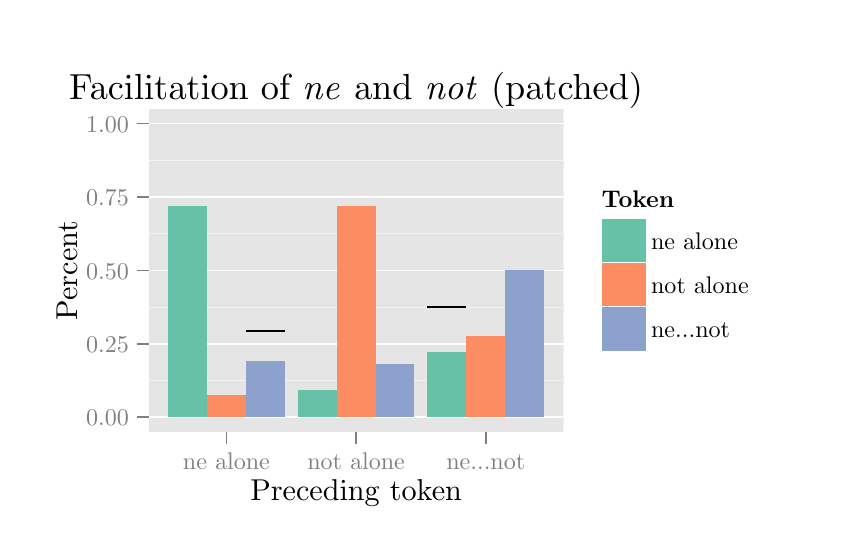
\begin{tikzpicture}[x=1pt,y=1pt]
\definecolor[named]{fillColor}{rgb}{1.00,1.00,1.00}
\path[use as bounding box,fill=fillColor,fill opacity=0.00] (0,0) rectangle (289.08,180.67);
\begin{scope}
\path[clip] (  0.00,  0.00) rectangle (289.08,180.67);
\definecolor[named]{drawColor}{rgb}{1.00,1.00,1.00}
\definecolor[named]{fillColor}{rgb}{1.00,1.00,1.00}

\path[draw=drawColor,line width= 0.6pt,line join=round,line cap=round,fill=fillColor] ( -0.00,  0.00) rectangle (289.08,180.68);
\end{scope}
\begin{scope}
\path[clip] ( 43.70, 34.60) rectangle (193.65,151.31);
\definecolor[named]{fillColor}{rgb}{0.90,0.90,0.90}

\path[fill=fillColor] ( 43.70, 34.60) rectangle (193.65,151.31);
\definecolor[named]{drawColor}{rgb}{0.95,0.95,0.95}

\path[draw=drawColor,line width= 0.3pt,line join=round] ( 43.70, 53.17) --
	(193.65, 53.17);

\path[draw=drawColor,line width= 0.3pt,line join=round] ( 43.70, 79.69) --
	(193.65, 79.69);

\path[draw=drawColor,line width= 0.3pt,line join=round] ( 43.70,106.22) --
	(193.65,106.22);

\path[draw=drawColor,line width= 0.3pt,line join=round] ( 43.70,132.74) --
	(193.65,132.74);
\definecolor[named]{drawColor}{rgb}{1.00,1.00,1.00}

\path[draw=drawColor,line width= 0.6pt,line join=round] ( 43.70, 39.90) --
	(193.65, 39.90);

\path[draw=drawColor,line width= 0.6pt,line join=round] ( 43.70, 66.43) --
	(193.65, 66.43);

\path[draw=drawColor,line width= 0.6pt,line join=round] ( 43.70, 92.95) --
	(193.65, 92.95);

\path[draw=drawColor,line width= 0.6pt,line join=round] ( 43.70,119.48) --
	(193.65,119.48);

\path[draw=drawColor,line width= 0.6pt,line join=round] ( 43.70,146.00) --
	(193.65,146.00);
\definecolor[named]{fillColor}{rgb}{0.40,0.76,0.65}

\path[fill=fillColor] ( 50.73, 39.90) rectangle ( 64.79,116.40);
\definecolor[named]{fillColor}{rgb}{0.99,0.55,0.38}

\path[fill=fillColor] ( 64.79, 39.90) rectangle ( 78.84, 47.92);
\definecolor[named]{fillColor}{rgb}{0.55,0.63,0.80}

\path[fill=fillColor] ( 78.84, 39.90) rectangle ( 92.90, 60.26);
\definecolor[named]{fillColor}{rgb}{0.40,0.76,0.65}

\path[fill=fillColor] ( 97.59, 39.90) rectangle (111.65, 49.68);
\definecolor[named]{fillColor}{rgb}{0.99,0.55,0.38}

\path[fill=fillColor] (111.65, 39.90) rectangle (125.70,116.18);
\definecolor[named]{fillColor}{rgb}{0.55,0.63,0.80}

\path[fill=fillColor] (125.70, 39.90) rectangle (139.76, 58.97);
\definecolor[named]{fillColor}{rgb}{0.40,0.76,0.65}

\path[fill=fillColor] (144.45, 39.90) rectangle (158.51, 63.36);
\definecolor[named]{fillColor}{rgb}{0.99,0.55,0.38}

\path[fill=fillColor] (158.51, 39.90) rectangle (172.56, 69.37);
\definecolor[named]{fillColor}{rgb}{0.55,0.63,0.80}

\path[fill=fillColor] (172.56, 39.90) rectangle (186.62, 93.08);
\definecolor[named]{drawColor}{rgb}{0.00,0.00,0.00}

\path[draw=drawColor,line width= 0.6pt,line join=round] (144.45, 79.69) --
	(158.51, 79.69);

\path[draw=drawColor,line width= 0.6pt,line join=round] (151.48, 79.69) --
	(151.48, 79.69);

\path[draw=drawColor,line width= 0.6pt,line join=round] (144.45, 79.69) --
	(158.51, 79.69);

\path[draw=drawColor,line width= 0.6pt,line join=round] ( 78.84, 71.14) --
	( 92.90, 71.14);

\path[draw=drawColor,line width= 0.6pt,line join=round] ( 85.87, 71.14) --
	( 85.87, 71.14);

\path[draw=drawColor,line width= 0.6pt,line join=round] ( 78.84, 71.14) --
	( 92.90, 71.14);
\end{scope}
\begin{scope}
\path[clip] (  0.00,  0.00) rectangle (289.08,180.67);
\definecolor[named]{drawColor}{rgb}{0.50,0.50,0.50}

\node[text=drawColor,anchor=base east,inner sep=0pt, outer sep=0pt, scale=  0.87] at ( 36.59, 36.74) {0.00};

\node[text=drawColor,anchor=base east,inner sep=0pt, outer sep=0pt, scale=  0.87] at ( 36.59, 63.27) {0.25};

\node[text=drawColor,anchor=base east,inner sep=0pt, outer sep=0pt, scale=  0.87] at ( 36.59, 89.79) {0.50};

\node[text=drawColor,anchor=base east,inner sep=0pt, outer sep=0pt, scale=  0.87] at ( 36.59,116.32) {0.75};

\node[text=drawColor,anchor=base east,inner sep=0pt, outer sep=0pt, scale=  0.87] at ( 36.59,142.84) {1.00};
\end{scope}
\begin{scope}
\path[clip] (  0.00,  0.00) rectangle (289.08,180.67);
\definecolor[named]{drawColor}{rgb}{0.50,0.50,0.50}

\path[draw=drawColor,line width= 0.6pt,line join=round] ( 39.43, 39.90) --
	( 43.70, 39.90);

\path[draw=drawColor,line width= 0.6pt,line join=round] ( 39.43, 66.43) --
	( 43.70, 66.43);

\path[draw=drawColor,line width= 0.6pt,line join=round] ( 39.43, 92.95) --
	( 43.70, 92.95);

\path[draw=drawColor,line width= 0.6pt,line join=round] ( 39.43,119.48) --
	( 43.70,119.48);

\path[draw=drawColor,line width= 0.6pt,line join=round] ( 39.43,146.00) --
	( 43.70,146.00);
\end{scope}
\begin{scope}
\path[clip] (  0.00,  0.00) rectangle (289.08,180.67);
\definecolor[named]{drawColor}{rgb}{0.50,0.50,0.50}

\path[draw=drawColor,line width= 0.6pt,line join=round] ( 71.81, 30.33) --
	( 71.81, 34.60);

\path[draw=drawColor,line width= 0.6pt,line join=round] (118.67, 30.33) --
	(118.67, 34.60);

\path[draw=drawColor,line width= 0.6pt,line join=round] (165.54, 30.33) --
	(165.54, 34.60);
\end{scope}
\begin{scope}
\path[clip] (  0.00,  0.00) rectangle (289.08,180.67);
\definecolor[named]{drawColor}{rgb}{0.50,0.50,0.50}

\node[text=drawColor,anchor=base,inner sep=0pt, outer sep=0pt, scale=  0.87] at ( 71.81, 21.16) {ne alone};

\node[text=drawColor,anchor=base,inner sep=0pt, outer sep=0pt, scale=  0.87] at (118.67, 21.16) {not alone};

\node[text=drawColor,anchor=base,inner sep=0pt, outer sep=0pt, scale=  0.87] at (165.54, 21.16) {ne...not};
\end{scope}
\begin{scope}
\path[clip] (  0.00,  0.00) rectangle (289.08,180.67);
\definecolor[named]{drawColor}{rgb}{0.00,0.00,0.00}

\node[text=drawColor,anchor=base,inner sep=0pt, outer sep=0pt, scale=  1.09] at (118.67,  9.94) {Preceding token};
\end{scope}
\begin{scope}
\path[clip] (  0.00,  0.00) rectangle (289.08,180.67);
\definecolor[named]{drawColor}{rgb}{0.00,0.00,0.00}

\node[text=drawColor,rotate= 90.00,anchor=base,inner sep=0pt, outer sep=0pt, scale=  1.09] at ( 17.85, 92.95) {Percent};
\end{scope}
\begin{scope}
\path[clip] (  0.00,  0.00) rectangle (289.08,180.67);
\definecolor[named]{fillColor}{rgb}{1.00,1.00,1.00}

\path[fill=fillColor] (203.12, 59.73) rectangle (266.36,126.18);
\end{scope}
\begin{scope}
\path[clip] (  0.00,  0.00) rectangle (289.08,180.67);
\definecolor[named]{drawColor}{rgb}{0.00,0.00,0.00}

\node[text=drawColor,anchor=base west,inner sep=0pt, outer sep=0pt, scale=  0.87] at (207.39,115.67) {\bfseries Token};
\end{scope}
\begin{scope}
\path[clip] (  0.00,  0.00) rectangle (289.08,180.67);
\definecolor[named]{drawColor}{rgb}{1.00,1.00,1.00}
\definecolor[named]{fillColor}{rgb}{0.95,0.95,0.95}

\path[draw=drawColor,line width= 0.6pt,line join=round,line cap=round,fill=fillColor] (207.39, 95.80) rectangle (223.29,111.70);
\end{scope}
\begin{scope}
\path[clip] (  0.00,  0.00) rectangle (289.08,180.67);
\definecolor[named]{fillColor}{rgb}{0.40,0.76,0.65}

\path[fill=fillColor] (207.39, 95.80) rectangle (223.29,111.70);

\path[] (207.39, 95.80) --
	(223.29,111.70);
\end{scope}
\begin{scope}
\path[clip] (  0.00,  0.00) rectangle (289.08,180.67);
\definecolor[named]{drawColor}{rgb}{1.00,1.00,1.00}
\definecolor[named]{fillColor}{rgb}{0.95,0.95,0.95}

\path[draw=drawColor,line width= 0.6pt,line join=round,line cap=round,fill=fillColor] (207.39, 79.90) rectangle (223.29, 95.80);
\end{scope}
\begin{scope}
\path[clip] (  0.00,  0.00) rectangle (289.08,180.67);
\definecolor[named]{fillColor}{rgb}{0.99,0.55,0.38}

\path[fill=fillColor] (207.39, 79.90) rectangle (223.29, 95.80);

\path[] (207.39, 79.90) --
	(223.29, 95.80);
\end{scope}
\begin{scope}
\path[clip] (  0.00,  0.00) rectangle (289.08,180.67);
\definecolor[named]{drawColor}{rgb}{1.00,1.00,1.00}
\definecolor[named]{fillColor}{rgb}{0.95,0.95,0.95}

\path[draw=drawColor,line width= 0.6pt,line join=round,line cap=round,fill=fillColor] (207.39, 64.00) rectangle (223.29, 79.90);
\end{scope}
\begin{scope}
\path[clip] (  0.00,  0.00) rectangle (289.08,180.67);
\definecolor[named]{fillColor}{rgb}{0.55,0.63,0.80}

\path[fill=fillColor] (207.39, 64.00) rectangle (223.29, 79.90);

\path[] (207.39, 64.00) --
	(223.29, 79.90);
\end{scope}
\begin{scope}
\path[clip] (  0.00,  0.00) rectangle (289.08,180.67);
\definecolor[named]{drawColor}{rgb}{0.00,0.00,0.00}

\node[text=drawColor,anchor=base west,inner sep=0pt, outer sep=0pt, scale=  0.87] at (225.28,100.58) {ne alone};
\end{scope}
\begin{scope}
\path[clip] (  0.00,  0.00) rectangle (289.08,180.67);
\definecolor[named]{drawColor}{rgb}{0.00,0.00,0.00}

\node[text=drawColor,anchor=base west,inner sep=0pt, outer sep=0pt, scale=  0.87] at (225.28, 84.68) {not alone};
\end{scope}
\begin{scope}
\path[clip] (  0.00,  0.00) rectangle (289.08,180.67);
\definecolor[named]{drawColor}{rgb}{0.00,0.00,0.00}

\node[text=drawColor,anchor=base west,inner sep=0pt, outer sep=0pt, scale=  0.87] at (225.28, 68.78) {ne...not};
\end{scope}
\begin{scope}
\path[clip] (  0.00,  0.00) rectangle (289.08,180.67);
\definecolor[named]{drawColor}{rgb}{0.00,0.00,0.00}

\node[text=drawColor,anchor=base,inner sep=0pt, outer sep=0pt, scale=  1.31] at (118.67,154.62) {Facilitation of \emph{ne} and \emph{not} (patched)};
\end{scope}
\end{tikzpicture}

    \caption{Predictions of the three-atom model, after applying a correction for adverbial uses of \emph{ne...not} constructions.}
    \label{fig:patch}
\end{figure}

After applying a correction derived from \textcite{Frisch1997}, we
obtain the graph in Figure~\ref{fig:patch}.  The black marks indicate
the original positions of the patched bars.\footnote{The other bars have
also been moved because of the patch, since in this model the bars are
constrained to sum to 100\%.}  As can be seen, the correction brings the
data in closer line with the predictions of the three-atom model.

\subsection{Further evidence against the two-atom model}
\label{sec:furth-evid-against}

\begin{figure}
    \centering
    % Created by tikzDevice version 0.6.2-92-0ad2792 on 2013-07-31 02:20:58
% !TEX encoding = UTF-8 Unicode
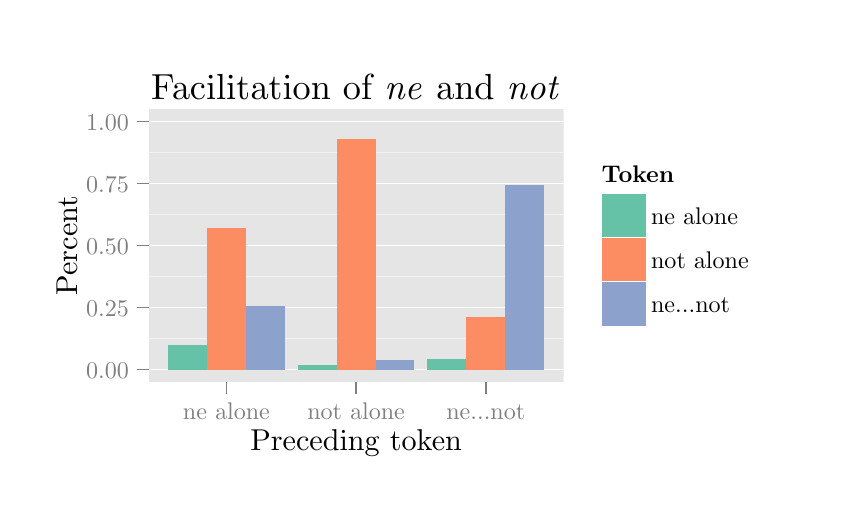
\begin{tikzpicture}[x=1pt,y=1pt]
\definecolor[named]{fillColor}{rgb}{1.00,1.00,1.00}
\path[use as bounding box,fill=fillColor,fill opacity=0.00] (0,0) rectangle (289.08,162.61);
\begin{scope}
\path[clip] (  0.00,  0.00) rectangle (289.08,162.61);
\definecolor[named]{drawColor}{rgb}{1.00,1.00,1.00}
\definecolor[named]{fillColor}{rgb}{1.00,1.00,1.00}

\path[draw=drawColor,line width= 0.6pt,line join=round,line cap=round,fill=fillColor] ( -0.00,  0.00) rectangle (289.08,162.61);
\end{scope}
\begin{scope}
\path[clip] ( 43.70, 34.60) rectangle (193.65,133.24);
\definecolor[named]{fillColor}{rgb}{0.90,0.90,0.90}

\path[fill=fillColor] ( 43.70, 34.60) rectangle (193.65,133.24);
\definecolor[named]{drawColor}{rgb}{0.95,0.95,0.95}

\path[draw=drawColor,line width= 0.3pt,line join=round] ( 43.70, 50.29) --
	(193.65, 50.29);

\path[draw=drawColor,line width= 0.3pt,line join=round] ( 43.70, 72.71) --
	(193.65, 72.71);

\path[draw=drawColor,line width= 0.3pt,line join=round] ( 43.70, 95.13) --
	(193.65, 95.13);

\path[draw=drawColor,line width= 0.3pt,line join=round] ( 43.70,117.55) --
	(193.65,117.55);
\definecolor[named]{drawColor}{rgb}{1.00,1.00,1.00}

\path[draw=drawColor,line width= 0.6pt,line join=round] ( 43.70, 39.08) --
	(193.65, 39.08);

\path[draw=drawColor,line width= 0.6pt,line join=round] ( 43.70, 61.50) --
	(193.65, 61.50);

\path[draw=drawColor,line width= 0.6pt,line join=round] ( 43.70, 83.92) --
	(193.65, 83.92);

\path[draw=drawColor,line width= 0.6pt,line join=round] ( 43.70,106.34) --
	(193.65,106.34);

\path[draw=drawColor,line width= 0.6pt,line join=round] ( 43.70,128.76) --
	(193.65,128.76);
\definecolor[named]{fillColor}{rgb}{0.40,0.76,0.65}

\path[fill=fillColor] ( 50.73, 39.08) rectangle ( 64.79, 47.87);
\definecolor[named]{fillColor}{rgb}{0.99,0.55,0.38}

\path[fill=fillColor] ( 64.79, 39.08) rectangle ( 78.84, 90.07);
\definecolor[named]{fillColor}{rgb}{0.55,0.63,0.80}

\path[fill=fillColor] ( 78.84, 39.08) rectangle ( 92.90, 61.94);
\definecolor[named]{fillColor}{rgb}{0.40,0.76,0.65}

\path[fill=fillColor] ( 97.59, 39.08) rectangle (111.65, 40.58);
\definecolor[named]{fillColor}{rgb}{0.99,0.55,0.38}

\path[fill=fillColor] (111.65, 39.08) rectangle (125.70,122.44);
\definecolor[named]{fillColor}{rgb}{0.55,0.63,0.80}

\path[fill=fillColor] (125.70, 39.08) rectangle (139.76, 42.36);
\definecolor[named]{fillColor}{rgb}{0.40,0.76,0.65}

\path[fill=fillColor] (144.45, 39.08) rectangle (158.51, 42.75);
\definecolor[named]{fillColor}{rgb}{0.99,0.55,0.38}

\path[fill=fillColor] (158.51, 39.08) rectangle (172.56, 58.08);
\definecolor[named]{fillColor}{rgb}{0.55,0.63,0.80}

\path[fill=fillColor] (172.56, 39.08) rectangle (186.62,105.76);
\end{scope}
\begin{scope}
\path[clip] (  0.00,  0.00) rectangle (289.08,162.61);
\definecolor[named]{drawColor}{rgb}{0.50,0.50,0.50}

\node[text=drawColor,anchor=base east,inner sep=0pt, outer sep=0pt, scale=  0.87] at ( 36.59, 35.92) {0.00};

\node[text=drawColor,anchor=base east,inner sep=0pt, outer sep=0pt, scale=  0.87] at ( 36.59, 58.34) {0.25};

\node[text=drawColor,anchor=base east,inner sep=0pt, outer sep=0pt, scale=  0.87] at ( 36.59, 80.76) {0.50};

\node[text=drawColor,anchor=base east,inner sep=0pt, outer sep=0pt, scale=  0.87] at ( 36.59,103.18) {0.75};

\node[text=drawColor,anchor=base east,inner sep=0pt, outer sep=0pt, scale=  0.87] at ( 36.59,125.59) {1.00};
\end{scope}
\begin{scope}
\path[clip] (  0.00,  0.00) rectangle (289.08,162.61);
\definecolor[named]{drawColor}{rgb}{0.50,0.50,0.50}

\path[draw=drawColor,line width= 0.6pt,line join=round] ( 39.43, 39.08) --
	( 43.70, 39.08);

\path[draw=drawColor,line width= 0.6pt,line join=round] ( 39.43, 61.50) --
	( 43.70, 61.50);

\path[draw=drawColor,line width= 0.6pt,line join=round] ( 39.43, 83.92) --
	( 43.70, 83.92);

\path[draw=drawColor,line width= 0.6pt,line join=round] ( 39.43,106.34) --
	( 43.70,106.34);

\path[draw=drawColor,line width= 0.6pt,line join=round] ( 39.43,128.76) --
	( 43.70,128.76);
\end{scope}
\begin{scope}
\path[clip] (  0.00,  0.00) rectangle (289.08,162.61);
\definecolor[named]{drawColor}{rgb}{0.50,0.50,0.50}

\path[draw=drawColor,line width= 0.6pt,line join=round] ( 71.81, 30.33) --
	( 71.81, 34.60);

\path[draw=drawColor,line width= 0.6pt,line join=round] (118.67, 30.33) --
	(118.67, 34.60);

\path[draw=drawColor,line width= 0.6pt,line join=round] (165.54, 30.33) --
	(165.54, 34.60);
\end{scope}
\begin{scope}
\path[clip] (  0.00,  0.00) rectangle (289.08,162.61);
\definecolor[named]{drawColor}{rgb}{0.50,0.50,0.50}

\node[text=drawColor,anchor=base,inner sep=0pt, outer sep=0pt, scale=  0.87] at ( 71.81, 21.16) {ne alone};

\node[text=drawColor,anchor=base,inner sep=0pt, outer sep=0pt, scale=  0.87] at (118.67, 21.16) {not alone};

\node[text=drawColor,anchor=base,inner sep=0pt, outer sep=0pt, scale=  0.87] at (165.54, 21.16) {ne...not};
\end{scope}
\begin{scope}
\path[clip] (  0.00,  0.00) rectangle (289.08,162.61);
\definecolor[named]{drawColor}{rgb}{0.00,0.00,0.00}

\node[text=drawColor,anchor=base,inner sep=0pt, outer sep=0pt, scale=  1.09] at (118.67,  9.94) {Preceding token};
\end{scope}
\begin{scope}
\path[clip] (  0.00,  0.00) rectangle (289.08,162.61);
\definecolor[named]{drawColor}{rgb}{0.00,0.00,0.00}

\node[text=drawColor,rotate= 90.00,anchor=base,inner sep=0pt, outer sep=0pt, scale=  1.09] at ( 17.85, 83.92) {Percent};
\end{scope}
\begin{scope}
\path[clip] (  0.00,  0.00) rectangle (289.08,162.61);
\definecolor[named]{fillColor}{rgb}{1.00,1.00,1.00}

\path[fill=fillColor] (203.12, 50.70) rectangle (266.36,117.14);
\end{scope}
\begin{scope}
\path[clip] (  0.00,  0.00) rectangle (289.08,162.61);
\definecolor[named]{drawColor}{rgb}{0.00,0.00,0.00}

\node[text=drawColor,anchor=base west,inner sep=0pt, outer sep=0pt, scale=  0.87] at (207.39,106.64) {\bfseries Token};
\end{scope}
\begin{scope}
\path[clip] (  0.00,  0.00) rectangle (289.08,162.61);
\definecolor[named]{drawColor}{rgb}{1.00,1.00,1.00}
\definecolor[named]{fillColor}{rgb}{0.95,0.95,0.95}

\path[draw=drawColor,line width= 0.6pt,line join=round,line cap=round,fill=fillColor] (207.39, 86.76) rectangle (223.29,102.66);
\end{scope}
\begin{scope}
\path[clip] (  0.00,  0.00) rectangle (289.08,162.61);
\definecolor[named]{fillColor}{rgb}{0.40,0.76,0.65}

\path[fill=fillColor] (207.39, 86.76) rectangle (223.29,102.66);

\path[] (207.39, 86.76) --
	(223.29,102.66);
\end{scope}
\begin{scope}
\path[clip] (  0.00,  0.00) rectangle (289.08,162.61);
\definecolor[named]{drawColor}{rgb}{1.00,1.00,1.00}
\definecolor[named]{fillColor}{rgb}{0.95,0.95,0.95}

\path[draw=drawColor,line width= 0.6pt,line join=round,line cap=round,fill=fillColor] (207.39, 70.86) rectangle (223.29, 86.76);
\end{scope}
\begin{scope}
\path[clip] (  0.00,  0.00) rectangle (289.08,162.61);
\definecolor[named]{fillColor}{rgb}{0.99,0.55,0.38}

\path[fill=fillColor] (207.39, 70.86) rectangle (223.29, 86.76);

\path[] (207.39, 70.86) --
	(223.29, 86.76);
\end{scope}
\begin{scope}
\path[clip] (  0.00,  0.00) rectangle (289.08,162.61);
\definecolor[named]{drawColor}{rgb}{1.00,1.00,1.00}
\definecolor[named]{fillColor}{rgb}{0.95,0.95,0.95}

\path[draw=drawColor,line width= 0.6pt,line join=round,line cap=round,fill=fillColor] (207.39, 54.96) rectangle (223.29, 70.86);
\end{scope}
\begin{scope}
\path[clip] (  0.00,  0.00) rectangle (289.08,162.61);
\definecolor[named]{fillColor}{rgb}{0.55,0.63,0.80}

\path[fill=fillColor] (207.39, 54.96) rectangle (223.29, 70.86);

\path[] (207.39, 54.96) --
	(223.29, 70.86);
\end{scope}
\begin{scope}
\path[clip] (  0.00,  0.00) rectangle (289.08,162.61);
\definecolor[named]{drawColor}{rgb}{0.00,0.00,0.00}

\node[text=drawColor,anchor=base west,inner sep=0pt, outer sep=0pt, scale=  0.87] at (225.28, 91.55) {ne alone};
\end{scope}
\begin{scope}
\path[clip] (  0.00,  0.00) rectangle (289.08,162.61);
\definecolor[named]{drawColor}{rgb}{0.00,0.00,0.00}

\node[text=drawColor,anchor=base west,inner sep=0pt, outer sep=0pt, scale=  0.87] at (225.28, 75.65) {not alone};
\end{scope}
\begin{scope}
\path[clip] (  0.00,  0.00) rectangle (289.08,162.61);
\definecolor[named]{drawColor}{rgb}{0.00,0.00,0.00}

\node[text=drawColor,anchor=base west,inner sep=0pt, outer sep=0pt, scale=  0.87] at (225.28, 59.75) {ne...not};
\end{scope}
\begin{scope}
\path[clip] (  0.00,  0.00) rectangle (289.08,162.61);
\definecolor[named]{drawColor}{rgb}{0.00,0.00,0.00}

\node[text=drawColor,anchor=base,inner sep=0pt, outer sep=0pt, scale=  1.31] at (118.67,136.55) {Facilitation of \emph{ne} and \emph{not}};
\end{scope}
\end{tikzpicture}

    \caption{Facilitation effects from 1350–1400.}
    \label{fig:later-evid}
\end{figure}

Another piece of evidence in favor of the three-atom model comes from
the later period of the change (1350–1400; N = 1617).  In
Figure~\ref{fig:later-evid}, we see that \emph{ne} facilitates
\emph{not} more strongly than \emph{ne ... not} does, which is never
expected to happen on the two-atom model.

\section{Conclusion}
\label{sec:conclusion}

The corpus persistence data presented here, interpreted as priming, are
inconsistent with the two-atom model and provide tenuous support for the
three-atom one.  It remains a subject of investigation how this fact
fits into the total picture of evidence about the change, which must
also include the evidence discussed by \textcite{Frisch1997} and
\textcite{wallage08}.

More broadly, the CRH is important because it provides a link between
frequency data attested in historical corpora and the mental
representations that underlie language and language change.  We would
like to suggest that persistence data constitute another, independent
source of linkage between these two domains.  The investigation of
persistence evidence can support and refine the conclusions of
quantitative studies of syntactic change.

\printbibliography

\end{document}
